\documentclass[12pt,a4paper]{ctexart}

\usepackage[a4paper,margin=2.5cm]{geometry}
\usepackage{setspace}
\usepackage{array}
\usepackage{longtable}
\usepackage{graphicx}
\usepackage{fancyhdr}
\usepackage{titling}
\usepackage{enumitem}
\usepackage{amsmath,amssymb}
\usepackage{booktabs}
\usepackage{caption}
\usepackage{float}
\usepackage{hyperref}
\usepackage{listings}
\usepackage[dvipsnames, svgnames, x11names]{xcolor}

\lstset{
	backgroundcolor=\color[rgb]{0.96,0.96,0.96},
	keywordstyle=\color{blue}\bfseries,
	identifierstyle=\color{black},
	commentstyle=\color[rgb]{0,0.6,0},
	stringstyle=\color[rgb]{0.58,0,0.82},
	basicstyle=\small\ttfamily,
	columns=fullflexible,
	breaklines=true,
	captionpos=t,
	tabsize=4,
	morekeywords={},
	emph={self},
	emphstyle=\bfseries\color{Rhodamine},
	frame=lines,
	framesep=1em,
	rulesepcolor=\color{red!20!green!20!blue!20},
	language=Python,
	numbers=left,
	showstringspaces=false,
	numberstyle=\footnotesize,
	extendedchars=false,
	xleftmargin=3em
}

\setlength{\parindent}{2em}
\setlength{\parskip}{0.5em}
\renewcommand{\arraystretch}{1.5}
\linespread{1.3}

\pagestyle{fancy}
\fancyhf{}
\cfoot{\thepage}
\renewcommand{\headrulewidth}{0pt}

% ===== 可修改信息 =====
\newcommand{\schoolname}{数学与统计学院}
\newcommand{\classname}{数学强基2301}
\newcommand{\studentid}{2233210080}
\newcommand{\studentname}{袁浩然}
\newcommand{\teachername}{孟德宇老师}
\newcommand{\labplace}{数学实验中心}
\newcommand{\experimenttitle}{PCA 算法消除噪声}
\newcommand{\schoolyear}{2023--2024学年\quad 第二学期}

\begin{document}

\begin{titlepage}
	\centering
	{
\includegraphics[scale=1]{figure1.jpg}}

	\vspace{1.8cm}

	{\heiti\zihao{-1} 机器学习\par}

	\vspace{2.2cm}

	{\zihao{3} 实验报告\par}

	\vspace{1.8cm}

	{\zihao{4} \schoolyear\par}

	\vspace{1.8cm}

	\renewcommand{\arraystretch}{2.0}
	\begin{tabular}{>{\raggedleft\arraybackslash}p{7cm} p{9cm}}
		学\hspace{2em}院： & \schoolname \\
		班\hspace{2em}级： & \classname \\
		学\hspace{2em}号： & \studentid \\
		姓\hspace{2em}名： & \studentname \\
		指导教师： & \teachername \\
		实验地点： & \labplace \\
	\end{tabular}

	\vfill
\end{titlepage}

\section*{实验四：PCA 算法消除噪声}

\section*{一、问题描述}
本次实验构造一个包含噪声的 4 维数据集，目标是利用 PCA 方法尽可能保留主要有效信息、压制随机噪声影响，并观察降噪前后数据质量变化。题目要求尽量不要直接调用现成 PCA 算法，因此本实验采用 NumPy 手写 PCA 的方式完成。

实验主要任务包括：
\begin{enumerate}
	\item 准备含噪数据；
	\item 手写 PCA 并提取主成分；
	\item 用低维表示重建原始数据实现降噪；
	\item 对比降噪前后的可视化与指标结果。
\end{enumerate}

\section*{二、算法原理}
PCA 的核心思想是将原始特征空间旋转到一组正交基上，使数据在前几个方向上具有最大方差。通常噪声更容易分散在小方差方向上，因此保留主要主成分并进行重建可以达到降噪目的。

设标准化后的数据为 $X\in\mathbb{R}^{n\times d}$，其协方差矩阵为：
\[
\Sigma = \frac{1}{n-1}X^TX
\]
对 $\Sigma$ 做特征分解，得到特征值与特征向量。将特征值从大到小排序后，取前 $k$ 个特征向量组成投影矩阵 $W_k$，则：
\[
Z = XW_k
\]
为低维表示；再做反变换：
\[
\hat{X} = ZW_k^T
\]
可得到去噪后的重建结果。

本实验中原始数据是 4 维，降到 2 维（$k=2$）后再重建，观察降噪效果。
另外，我对 PCA 原始论文进行了复现，复现笔记同样放在文件夹中。

\section*{三、实验步骤与实现细节}
\begin{enumerate}
	\item 先构造 2 个潜在变量，并线性组合成 4 维“干净数据”；
	\item 在每个特征上叠加高斯噪声，得到含噪数据；
	\item 对含噪数据做标准化；
	\item 手写 PCA：协方差矩阵、特征分解、排序选主成分；
	\item 将数据投影到前 2 个主成分，再逆变换到原空间得到去噪数据；
	\item 用 MSE 和逐特征相关系数评估去噪效果；
	\item 绘制三类图：数据对比散点图、方差贡献率图、相关系数对比图。
\end{enumerate}

\section*{四、核心代码}
下面给出核心实现片段。完整代码包含数据生成、评估和可视化。

\begin{lstlisting}
class PCAFromScratch:
	def __init__(self, n_components=2):
		self.n_components = n_components
		self.mean_ = None
		self.components_ = None
		self.eigenvalues_ = None
		self.explained_variance_ratio_ = None

	def fit(self, x):
		self.mean_ = np.mean(x, axis=0)
		x_centered = x - self.mean_
		cov = np.dot(x_centered.T, x_centered) / (x_centered.shape[0] - 1)
		eigenvalues, eigenvectors = np.linalg.eigh(cov)

		sorted_indices = np.argsort(eigenvalues)[::-1]
		eigenvalues = eigenvalues[sorted_indices]
		eigenvectors = eigenvectors[:, sorted_indices]

		self.eigenvalues_ = eigenvalues
		self.components_ = eigenvectors[:, : self.n_components]
		self.explained_variance_ratio_ = eigenvalues / np.sum(eigenvalues)
		return self

	def transform(self, x):
		x_centered = x - self.mean_
		return np.dot(x_centered, self.components_)

	def inverse_transform(self, z):
		return np.dot(z, self.components_.T) + self.mean_

def main():
	x_clean, x_noisy = generate_noisy_dataset(n_samples=200, random_state=7)
	scaler = StandardScaler()
	x_noisy_std = scaler.fit_transform(x_noisy)

	pca = PCAFromScratch(n_components=2)
	z = pca.fit_transform(x_noisy_std)
	x_recon_std = pca.inverse_transform(z)
	x_denoised = scaler.inverse_transform(x_recon_std)
\end{lstlisting}

\section*{五、实验结果与分析}
实验运行后，含噪数据经过 PCA 降维重建得到去噪结果。对比可以看到，去噪后样本分布整体更接近干净数据的主结构，离散噪声点明显减少。

从指标上看：
\begin{enumerate}
	\item $\mathrm{MSE}(\text{clean},\text{denoised})$ 小于 $\mathrm{MSE}(\text{clean},\text{noisy})$，说明重建后的误差下降；
	\item 各特征与干净数据的相关系数在去噪后普遍提升，说明有效信息保留更好；
	\item 前两个主成分解释了主要方差信息，因此取 2 维重建在本实验中是有效的。
\end{enumerate}

\begin{figure}[H]
	\centering
	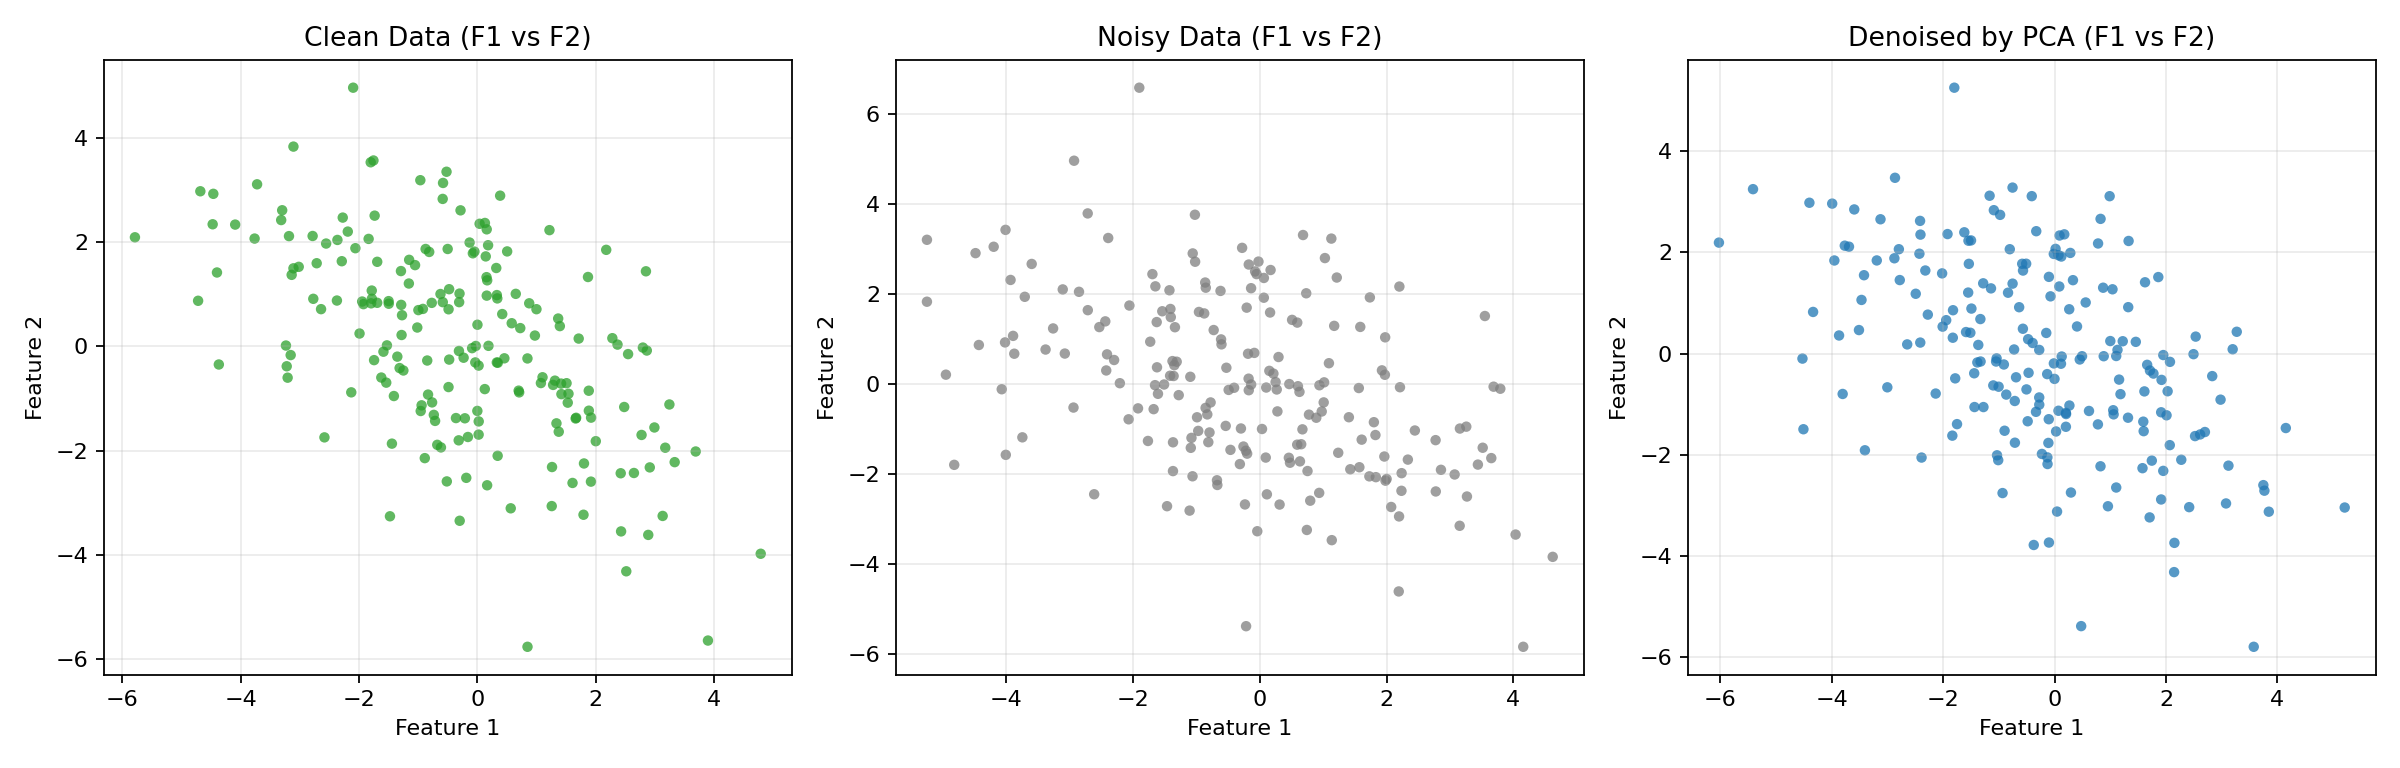
\includegraphics[width=0.95\textwidth]{data_compare.png}
	\caption{干净数据、含噪数据与 PCA 去噪后数据对比（F1-F2 平面）}
\end{figure}

\begin{figure}[H]
	\centering
	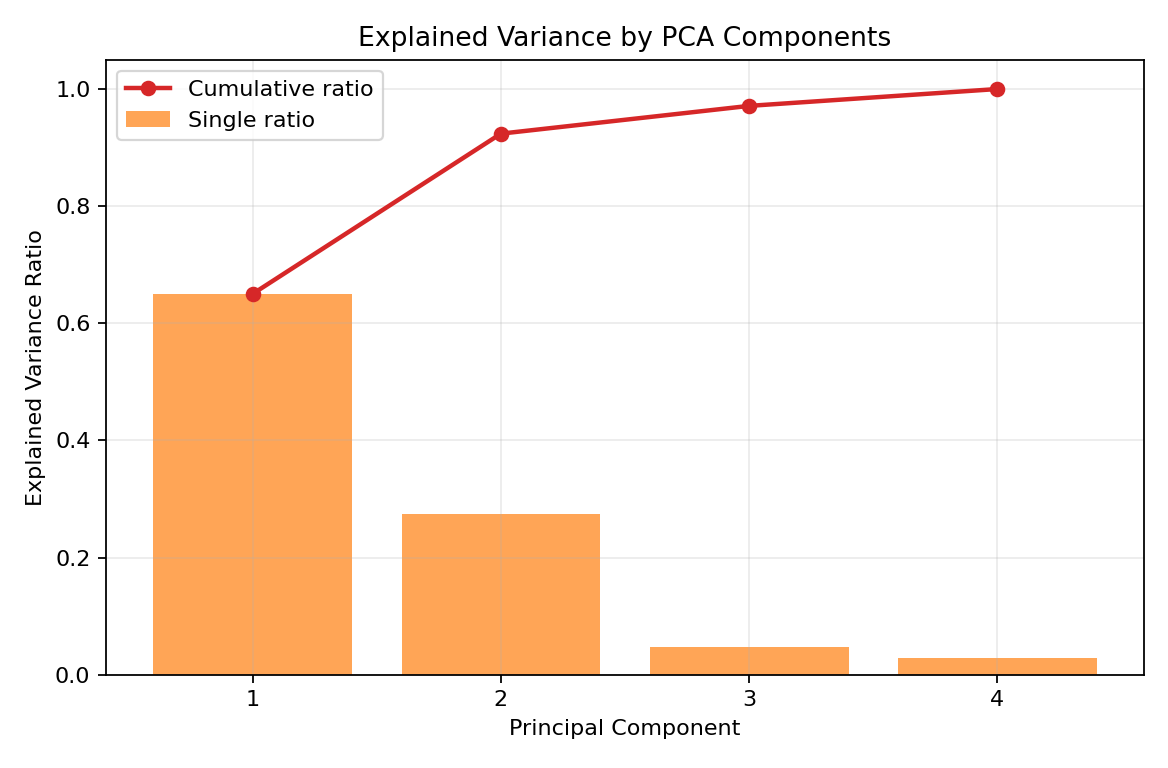
\includegraphics[width=0.78\textwidth]{variance_curve.png}
	\caption{PCA 各主成分方差贡献率与累计贡献率}
\end{figure}

\begin{figure}[H]
	\centering
	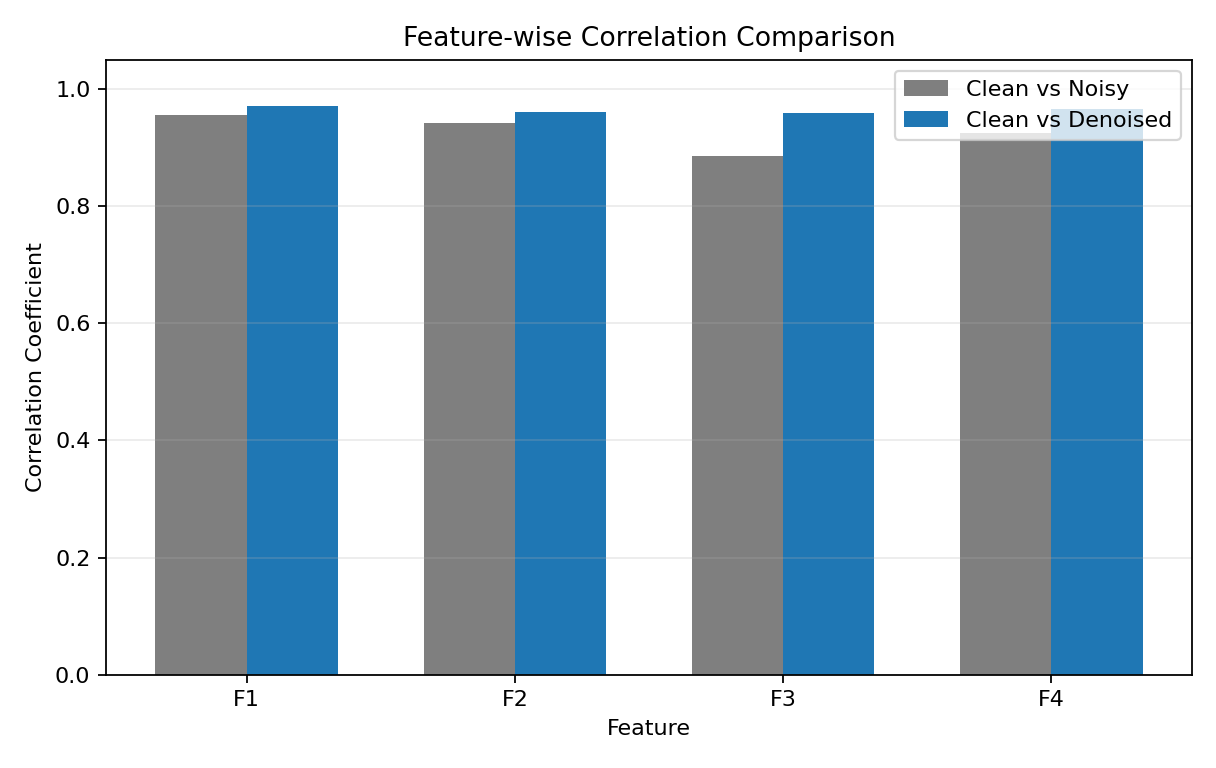
\includegraphics[scale=0.5]{corr_compare.png}
	\caption{各特征相关系数对比（去噪前后）}
\end{figure}

\section*{六、实验总结}
本次实验按要求完成了手写 PCA 去噪流程：数据构造、特征分解、降维重建、效果评估和可视化展示。实验结果表明，PCA 在保留主要结构信息的同时，确实能够降低随机噪声带来的干扰。


\end{document}